\chapter{Fundamentação Teórica}\label{cap_exemplos}
\section{Sistemas de Recomendação}
Sistemas de recomendação são ferramentas de softwares e técnicas que fornecem sugestões de itens para serem utilizados por um usuário\cite{ricci2011introduction}. Alguns exemplos dessa ferramenta são os sistemas de recomendação de vídeos, músicas e livros que são muito utilizados em \textit{streamings} e \textit{e-commerce}.

A principal motivação para uso dessa ferramenta é a grande quantidade de informação disponível para os usuários. Essa grande quantidade faz com que os usuários normalmente tenha uma alto número de itens(como músicas, filmes e livros) para escolher, e isso pode ser positivo pelo fato de que o usuário vai ter muita liberdade para escolher. 

Porém, esse excesso de alternativas aumenta a expectativa do usuário sobre a sua escolha e isso acaba gerando uma paralisia e não sensação de liberdade, esse problema é conhecido como Paradoxo da Escolha\cite{schwartz2004paradox}.

Para evitar esse problema, os sistemas de recomendação são utilizados, esses sistemas são utilizados como filtros que selecionam os itens que tenham uma maior chance de ser escolhido pelo usuário. Devido a isso, diversos benefícios podem ser identificados a partir do uso dessas ferramentas:
\begin{itemize}
    \item Aumento da venda,
    \item Maior diversidade nos itens vendidos,
    \item Aumento da satisfação dos usuários,
    \item Aumento da fidelidade dos usuários,
    \item Maior entendimento das preferências dos usuários.
\end{itemize}



Os sistema de recomendações são divididos em duas categorias     principais: sistemas de recomendações personalizados e não personalizados\cite{jain2015trends}.

Sistemas de recomendação personalizados utilizam o histórico do usuário para recomendar itens cujo o usuário tenha mais chance de gostar, os sistemas não personalizados não levam em consideração o histórico do usuário para executar a recomendação, nele, apenas os itens mais bem avaliados são recomendados\cite{khatwani2016building}.

Os  Sistemas de recomendação, normalmente, utilizam três tipos de informação para executar as recomendações\cite{ricci2011introduction}:
\begin{itemize}
    \item Itens: São os objetos que são recomendados, podem ser caracterizados pela sua complexidade e seu valor ou utilidade. O valor de um item muitas vezes é representado como a relevância daquele item para o usuário, essa relevância leva em conta diversos fatores, como o gosto do usuário e o custo para obter esse item.
    \item Usuários: São aqueles cujo o sistema irá recomendar os itens, deve ser levado em conta o fato os usuários podem ter diferentes tipos e características. Os Sistemas Recomendação buscam explorar todas representações possíveis do usuário, desde uma simples listas de avaliação até complexas representações vetoriais.
    \item Transações: São interações entre o usuário e o sistema de recomendação. Um exemplo de transação é a avaliação de um usuário sobre um item, tem diversos tipos de avaliação, mas as comuns são as numéricas (ex: notas de filmes do IMDB), as ordinais (ex: "Concordo Fortemente", " Concordo", "Neutro", "Discordo", "Discordo Totalmente"), binárias (ex:"Gostei" e "Não gostei") e unárias(ex: Indicativo de que o usuário observou o item).
\end{itemize}
Existem diversos tipos de técnicas para recomendações de itens, nas seções abaixo serão descritas as técnicas mais comuns.
\subsection{Baseada em Conteúdo}
Essa técnica busca analisar um conjunto de documentos ou/e descrições de itens previamente avaliado por um usuário, e construir um modelo dos interesses do usuário, baseado nas características dos objetos avaliados pelo usuário\cite{lops2011content}. Sistemas de recomendação baseados em conteúdo, normalmente, são projetados para explorar cenários em que os itens podem ser descritos como um conjunto de atributos\cite{aggarwal2016recommender}.

O processo de recomendação nessa técnica possui 3 componentes: análise do conteúdo,  aprendizado do perfil e a filtragem\cite{lops2011content}. O seu diagrama de fluxo pode ser visto na Figura~\ref{fig:cb}.

\begin{figure}[h!]
   
    \centering
    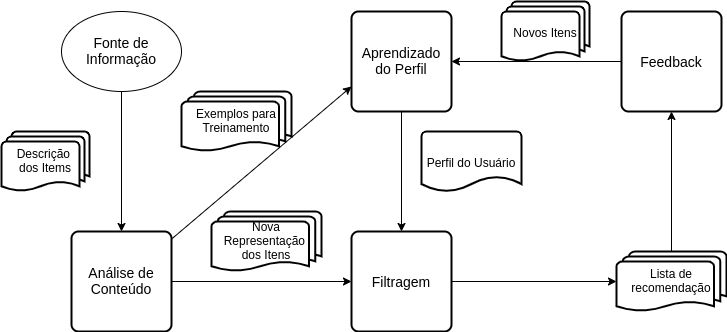
\includegraphics[width=12cm]{Imagens/content-based.png}
   \caption{Diagrama de fluxo de um sistema de recomendação baseado em conteúdo.}
    \label{fig:cb}
    
\end{figure}
\subsubsection{Análise de Conteúdo}
O processo de recomendação é inicializado com o componente de análise de conteúdo, que irá receber como entrada o conjunto de dados contendo as descrições dos itens que serão utilizados na recomendação.

Neste componente, os itens são analisados utilizando extração de características, gerando uma nova representação deste item. Essa nova representação será utilizada como entrada dos outros dois componentes.

Normalmente,  as informações dos itens não contém apenas dados numéricos, em muitos casos, os itens contém muitas informações textuais. 

Portanto, uma importante tarefa desse componente de Análise de Conteúdo, é o uso de técnicas para extração de características de textos. Existem diversas técnicas para extrair valores numéricos de textos, as mais populares são as seguintes:
\begin{itemize}
    \item \textbf{TF-IDF}: Essa técnica busca transformar cada texto (também chamado de documento) em um vetor, onde cada posição desse vetor é associado a um termo e o seu valor corresponde a um peso(chamado de tf-idf) que equivale a importância deste termo para o documento\cite{schutze2008introduction}.
    
    Esse peso é uma composição de duas medidas: TF(\textit{Term frequence}, em inglês) e IDF(\textit{Inverse document frequency}, em inglês). TF é uma medida que corresponde a quantidade de ocorrências de um termo em um documento \cite{schutze2008introduction}, normalmente denotada por \(tf_{t,d}\), onde \(t\) é o termo e \(d\) é o documento. Já o IDF é calculada com base em outra medida,  \(df\)(\textit{Document frequency}, em inglês), que corresponde a quantidade documentos que contém um termo. A equação do IDF é dada da seguinte forma:
    \begin{equation}
        idf_t = \log(\frac{N}{df})
    \end{equation}
    
    Onde N é o número total de documentos. Logo, pode-se afirmar que esta medida dá um maior grau de importância para termos que aparecem em poucos documentos. Então, a o valor do tf-idf é dado da seguinte forma:
    \begin{equation}
        \mbox{tf-idf}_{t, d} = tf_{t,d} \times idf_t 
    \end{equation}
    A partir dessa equação, três princípios básicos desse medida podem observados. O primeiro é que termos que ocorrem muito em um documento e aparecem em poucos documentos, são muito importantes para aquele documento. O segundo é que termos que aparecem em muitos documentos ou que aparece poucas vezes em um documento, tem pouca importância. O terceiro é que se o termo aparece em todos os documentos ele vai ser pouco relevante para todos os documentos.
    
    \item \textbf{Word2Vec}: É uma técnica que busca aprender representações vetoriais de palavras a partir de uma grande quantidade de dados textuais \cite{mikolov2013distributed}, portanto, esse método não pode ser usado diretamente para gerar um vetor de um texto, para isso, pode ser utilizar técnicas de agregação de vetores, como a soma de vetores. Word2Vec corresponde a uma extensão do método Skip-Gram, esse método busca criar representações vetoriais de palavras que seja útil para prever palavras próximas em uma sentença ou documento \cite{mikolov2013efficient}.
    
    O objetivo do Skip-Gram, dado uma sequencia de palavras \(w_1, w_2, w_3, ..., w_T\), é maximizar a probabilidade logarítmica média.
    \begin{equation}
        \frac{1}{T} \sum_{t=1}^{T}\sum_{-c \leq j \leq c, j \neq 0} \log p(w_{t+j} | w_t)
    \end{equation}
    A principal diferença entre o Skip-gram e WordVec está na definição do \(p(w_{t+j} | w_t)\), onde, no Skip-gram é uma função \textit{softmax}, que é definido da seguinte forma:
    \begin{equation}
        p(w_{O} | w_I) = \frac{\exp(v'_{w_O}^{T} v_{w_I})}{\sum_{w=1}^{W} \exp(v'_{w}^{T} v_{w_I})}
    \end{equation}
    Onde \(v_{w}\) e \(v'_{w}\) são as representações vetoriais de entrada e saída da palavra \(w\), respectivamente. No Word2Vec, duas definições para o calculo de \(p(w_{t+j} | w_t)\), a primeira é utilizando o \textit{softmax} hierárquico, que é uma forma mais eficiente de calcular o \textit{softmax}. 
    
    No \textit{softmax} hierárquico, é utilizado uma árvore binária para representar a distribuição de probabilidade, onde cada nó contém a probabilidade dos nós filhos e os nos folhas representam as palavras do dicionário \cite{mikolov2013distributed}. O calculo do \textit{softmax} hierárquico é definido da seguinte forma:
    \begin{equation}
        p(w | w_I) = \prod_{j=1}^{L(w)-1} \sigma([[n(w,j + 1) = ch(n(w,j))]] \cdot v'_{n(w, j)}^T v_{w_{I}})
    \end{equation}
    
    Onde \(n(w, j)\) é o j-ésimo nó do caminho entre a raiz e w, \(L(w)\) é o tamanho deste caminho, \(ch(n)\) é um nó filho arbitrário, \([[x]]\) é um função que retorna 1 caso x seja verdadeiro e -1 caso contrário, e \(\sigma(x)\) é a função sigmoid.
    
    A outra forma que o Word2Vec utiliza para calcular o \(p(w_{t+j} | w_t)\) é a partir de  Amostragem Negativa \cite{mikolov2013distributed}, que é definida da seguinte forma:  
    \begin{equation}
        p(w | w_I) = \log \sigma(v'_{w_{O}}^{T} v_{w_{I}}) + \sum_{i=1}^{k} \mathop{\mathbb{E}}_{w_i \sim P_n(w)} [ \log \sigma(-v'_{w_{i}}^{T} v_{w_{I}})]
    \end{equation}
    \item \textbf{Doc2Vec}: Essa técnica busca criar representações vetoriais para textos, ela é baseada em técnicas que aprendem representações de palavras para palavras próximas em uma frase ou texto \cite{le2014distributed}. Nesse método, para prever a próxima palavra em um texto, são utilizados os vetores das palavras anteriores a esta e o vetor que representa os documentos, para isso os vetores são agregado utilizando concatenação ou agregação. O framework do Doc2Vec pode ser visto na Figura \ref{fig:framework_doc2vec}.
    
    \begin{figure}[h!]
    \centering
    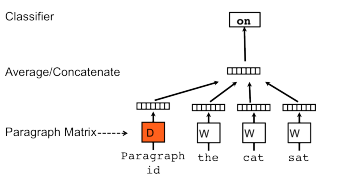
\includegraphics[width=12cm]{Imagens/framework_doc2vec.png}
    \caption{Diagrama de fluxo de um sistema de recomendação baseado em conteúdo.}
    \label{fig:framework_doc2vec}
    \end{figure}
    
\end{itemize}

O analisador de conteúdo processará esses dados e, com as técnicas de extração de características, gerará um novo conjunto de dados que conterá as novas representações dos itens.


\subsubsection{Aprendizado de Perfil}
Após a criação do conjunto de dado contendo as novas representação dos itens, é iniciado o processo de coleta de dados sobre as avaliações feitas pelos usuários sobre os itens. As avaliações podem ser obtidas de algumas formas, como avaliações numéricas, feedback implícito(e.g. ações do usuário), opiniões textuais. Essas avaliações são convertidas em uma avaliação no formato numérico\cite{aggarwal2016recommender}.

Com isso, são construídos conjunto de dados para cada usuário contendo as representações dos itens avaliados por esses usuários, cada item será rotulado pela avaliação do item feita pelo usuário. O componente de aprendizado de perfil receberá esses conjuntos de dados como entrada e criará um perfil para cada usuário, esse perfil representará os gostos do usuário.

O aprendizado de perfil coleta dados que representam as preferências do usuário, com esses dados, o componente tenta generalizar esses dados utilizando aprendizado de máquina para regressão, pois o valor que o modelo deve estimar é real. Existem diversas técnicas de aprendizado de máquina porém, as mais utilizadas são as seguintes:
\begin{itemize}
    \item \textbf{Regressão Linear}: Esse é o modelo mais simples para regressão. Esse modelo, tem como proposito, modelar a relação entre as variáveis de entrada \(X = x_1, x_2, ..., x_m\) e a variável alvo y com uma combinação linear,  \cite{bishop2006pattern}:
    \begin{equation}
        y = w_0 + w_1 * x_1 + w_2 * x_2 + ... + w_m * x_m = Xw
    \end{equation}
    Com isso, o modela tentar encontrar, ou aprender, os coeficientes \(w = w_0, w_1, w_2, ..., w_m\), também chamados de pesos, para que minimize a seguinte função de custo, chamada de erro quadrático:
     \begin{equation}
        L(X, w) = || Xw - y ||_{2}^{2}
    \end{equation}
    Uma forma utilizada para otimizar o vetor de pesos \(w\) é a partir do método de descida de gradiente estocástica, onde, dado um conjunto de vetores de entrada \(X^{(1)}, X^{(2)}, ..., X^{(n)}\) e o somatório da função de erro sobre o conjunto de vetores \(E(w) = \sum_{i=1}^{n} L(X^{(i)}, w)\) e uma taxa de aprendizado \(\alpha\), é executado um processo iterativo, onde a cada iteração t o vetor de pesos é alterado da seguinte forma:
    \begin{equation}
        w^{(t+1)} = w^{(t)} + \alpha * \Delta E 
    \end{equation}
    \item \textbf{Regressão Logística}: A regressão logística é uma extensão do regressão linear, onde a relação entre as variáveis não definidas por uma combinação linear, e sim, pela equação abaixo:
    \begin{equation}
        y = \phi(Xw)
    \end{equation}
    Onde, \(\phi\) é a função logística, definida da seguinte forma:
    \begin{equation}
        \phi(a) = \frac{1}{1 + \exp(-a)}
    \end{equation}
    \item \textbf{Modelo Ridge}: Esse modelo é uma variação modelo de regressão que busca resolver uma dificuldades desses modelos, que é o \textit{overfitting}, que quando o modelo fica superespecializado nos dados de treinamento e não consegue generalizar para dados novos\cite{Goodfellow-et-al-2016}.
    
    Para isso o modelo utiliza uma penalidade na função de custo, para que vetores pesos com valores menores tenham preferência no processo de otimização\cite{Goodfellow-et-al-2016}, esse penalidade é chamada de regularização. No modelo Ridge é utilizado a norma \(l^2\) como regularização \cite{scikit-learn}, assim a função de erro fica da seguinte forma:
    \begin{equation}
        l(w) = ||y - Xw||^2_2 + \alpha * ||w||^2_2
    \end{equation}
    \item \textbf{Modelo Lasso}: Esse modelo tem uma abordagem semelhante ao modelo Ridge. Porém, nesse modelo, a regularização é dada pela norma \(l^1\) \cite{scikit-learn}, dessa forma a função de erro desse modelo é a seguinte:
    \begin{equation}
        l(w) = ||y - Xw||^2_2 + \alpha * ||w||_1s
    \end{equation}
    \item \textbf{Elastic Net}: Esse modelo corresponde a uma combinação dos modelos Ridge e Lasso, onde a regularização é dada pela soma ponderada das normas \(l^1\) e \(l^2\) \cite{scikit-learn}. A função de custo do Elastic Net pode ser vista na equação abaixo.
    \begin{equation}
        l(w) = \frac{1}{2*n} * ||y - Xw||^2_2 +  \alpha * ||w||_1 +  \beta * ||w||^2_2 
    \end{equation}
    \item \textbf{\textit{Gradient Boosting Regressor}(GBR)}: Esse método busca construir um modelo a partir de um conjunto de modelos simples, usualmente os modelos utilizados são arvores de decisão, a construção do modelo é dada pela soma dos modelos mais simples \cite{friedman2002stochastic}.
\end{itemize}

\subsubsection{Filtragem}
Dados os perfis gerados pelo componente de Aprendizado de Perfil, o componente de Filtragem tenta prever quais itens cada usuário poderá se interessar. Esse componente, normalmente, gera uma lista ordenada dos itens mais relevantes para o usuário\cite{lops2011content}. 

A filtragem explora o perfil do usuário para sugerir itens relevantes, comparando a representação do perfil do usuário com a representação do item. O resultado é um julgamento de relevância utilizando métricas de similaridade.


Como o gosto do usuário tende a mudar com o passar do tempo, é necessário que todos os componentes sejam atualizados com base em \textit{feedbacks} dos usuários sobre os itens recomendados.
 
\subsubsection{Vantagem e desvantagens}

Algumas vantagens que podem ser identificadas nessa técnica é independência, com relação aos usuários do sistema, ao recomendar itens a um usuário. Além disso, o sistema será capaz de recomendar itens para um usuário com gostos únicos\cite{jain2015trends}. Outra vantagem desse tipo de abordagem é a capacidade de recomendar itens que foram pouco avaliados, já que o sistema depende apenas da representação do item.

Porém, esses sistemas são limitados pelas representação definida para o item, apresentando dificuldade para analisar itens mais complexos. Além disso, esses sistemas também tendem a ficar super especializados e não conseguem lidar com novos usuários, que fizeram poucas avaliações\cite{lops2011content}.

\subsection{Filtro Colaborativo (CF)}
Nesta técnica os itens são recomendados com base no gosto de um grupo de pessoas que fizeram boas avaliação de itens parecidos anteriormente. A premissa básica dessa técnica é que pessoas que gostaram da mesmas coisas no passado, também vão gostar de coisas parecidas no futuro\cite{shah2017recommender}.

Os algoritmos de CF  representam os dados que relacionam usuários e itens como uma matriz de avaliação A, onde cada elemento \(a_{i,j}\) da matriz é a avaliação do usuário \(u_i\) sobre o item \(i_j\)\cite{sarwar2001item}.

No momento da predição de uma avaliação de um usuário os CF tentam levar em consideração fatores que não dependem modelagem feita pelo sistema, esses fatores são chamados de vieses, e ele são somados em um única variável \(b_{ui}\), chamado de viés do preditor, que é dada da seguinte forma:
\begin{equation}
    b_{ui} = \upmu + b_u + b_i 
\end{equation}

Onde \(\upmu\) é a média de todas avaliações obtidas pelo sistema, \(b_u\) e \(b_i\) são os desvios das avaliações do usuário e do item, respectivamente.

Os CF são divididos em duas classes de algoritmos, baseado em vizinhança e baseado em modelos \cite{koren2015advances}.

\subsubsection{Baseado em vizinhança}
Nos CF baseado em vizinhança, as avaliações dos  usuários sobre os itens, que estão armazenados, são diretamente utilizadas no processo de recomendação. Essa classe pode ser dividida em duas técnicas, baseadas em itens e baseada em usuários. 
\begin{itemize}
    \item Baseado em  usuários: Esse tipo sistema calcula o nível de interesse do usuário \(u\) por um item \(i\) utilizando as avaliações desse item por um grupo de usuários, chamados de vizinhos. Esses vizinhos são os usuários que que fizeram avaliações de itens parecidas com as  avaliações do usuário \(u\).
    \item Baseados em itens: Esse sistema estima a avaliação do usuário u para o item \(i\) baseado em outras avaliações de  \(u\) para itens parecidos com \(i\). 

\end{itemize}
Na forma mais tradicional da implementação desses métodos, é construído uma matriz de similaridade (entre itens ou usuários, dependendo da abordagem), onde cada entrada dessa matriz corresponde a,no caso do método baseado em usuários, similaridade das avaliações dos usuários para os itens (sendo  que, quando o item não foi avaliado, é atribuído uma nota 0), e no caso do método baseado em itens, é a similaridade das avaliações que os itens receberam de todos os usuários.

Nas equações \ref{sim_item} e \ref{sim_user} podem ser vista o calculo da similaridade (utilizando a similaridade do cosseno) para o método baseado em itens e o baseado em usuários, respectivamente.

\begin{equation}
\label{sim_item}
    sim(i_a, i_b) = \frac{\sum_{u} r_{ui_a} * r_{ui_b}}{(\sum_{u} r_{ui_a}^{2}) \cdot (\sum_{u} r_{ui_b}^{2}) }
\end{equation}
\begin{equation}
\label{sim_user}
    sim(u_a, u_b) = \frac{\sum_{i} r_{u_ai} * r_{u_bi}}{(\sum_{i} r_{u_ai}^{2}) \cdot (\sum_{i} r_{u_bi}^{2}) }
\end{equation}

A partir do calculo da matriz de similaridade, o cálculo da possível avaliação que o usuário u daria para o item i é dada da seguinte forma(sendo que ):
\begin{equation}
\label{r_user_cf}  
r_{ui} = b_{ui} + \sum_{i'}^{N_u(i)} sim(u, u')*r(u, i') 
\end{equation}
\begin{equation}
\label{r_item_cf}  
r_{ui} = b_{ui} + \sum_{i'}^{N_i(u)} sim(u, u')*r(u', i) 
\end{equation}
Sendo, que a equação \ref{r_item_cf} é para estimar a avaliação no método baseado em itens, a equação \ref{r_item_cf} é para a baseado em usuário, \(N_u(i)\) são itens mais similares  ao item \(i\) que foram avaliado pelo usuário \(u\) e \(N_i(u)\) são os usuários mais similares ao usuário \(u\) que avaliaram o item \(i\).
\subsubsection{Baseado em modelo}
Os métodos baseado em modelo, diferentemente do baseado em vizinhança, buscam criar um modelo preditivo com base nas avaliações armazenadas. Esse método tenta lidar com o problema de ter muita informação  para ser processada, o que requer muito poder computacional\cite{thido2010}.

Os métodos mais comuns desse tipo de técnica são os modelos baseados em fatoração de matriz. Esse método mapeia os usuários e os itens para um novo espaço latente de  dimensionalidade \(f\), de tal forma que as avaliações do usuário sobre o item se transforme em um produto interno nesse espaço \cite{koren2015advances}. Uma ilustração desse método pode ser visto na Figura \ref{fig:matrix_fac}.
\begin{figure}[h!]
    \centering
    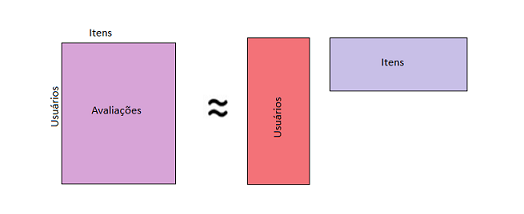
\includegraphics[width=14cm]{Imagens/matrix_fac.png}
    \caption{Fatoração de Matriz}
    \label{fig:matrix_fac}
\end{figure}

Dessa forma, cada item \(i\)é representado por um vetor \(q_i\) e cada usuário \(u\) é representado por um vetor \(p_u\), sendo que \(q_i, p_u \in \R \), então, como o produto interno entre esses vetores representam a relação entre o usuário e o item, então, a possível avaliação que o usuário poderia da para o item, pode ser calculada  da seguinte forma:
\begin{equation}
    r_{ui} = b_{ui} + q_{i}^{T} p_u 
\end{equation}
\subsection{Baseado em Conhecimento}
Nesse tipo de sistema as avaliações não é a principal fonte de informação para as recomendação, e sim com base medidas de similaridades que que obtidas a partir dos requisitos dos usuários e de descrições dos itens. O cálculo dessa medida é feito a partir do uso de bases de conhecimento que contém regras e funções para cálculo de similaridade\cite{aggarwal2016recommender}. 

Portanto, diferente dos os métodos anteriores, os sistemas baseado em conhecimento não faz recomendação a partir de ações passadas do usuário, esse tipo de sistema recomenda com base nas especificações do usuário.

Devido a independência da avaliação do usuário, esse sistema é utilizado para recomendação de itens que são comprado poucas vezes, como casas, carros e itens de luxo.
\subsection{Demográfica}
Nesse tipo de sistema, além da avaliação dos itens, as informação demográficas dos usuários  são utilizadas para identificar usuários similares para auxiliar no processo de recomendação\cite{aggarwal2016recommender}. A suposição desse método é que diferentes recomendações podem ser geradas para diferentes nichos demográficos\cite{ricci2011introduction}.
\section{Otimização Multiobjetivo}
Um problema de otimização multiobjetivo (MOP, do inglês \textit{Multi-Objective Optimization}) é um problema onde  o propósito é otimizar duas ou mais funções objetivos, podendo ser tanto a maximização dessas funções quanto a minimização\cite{coello2007evolutionary}. 

Uma solução de MOP minimiza (ou maximiza) os componentes de um vetor f(x) onde x é um vetor de variáveis de decisão n-dimensional, x = (x$_{1}$,..., x$_{n}$), a partir de um universo $\Omega$. O universo $\Omega$ contém todo x possível que pode ser utilizado para satisfazer uma avaliação de f(x). $\Lambda$ é o espaço do vetor das funções objetivo para o problema.

Neste tipo de problema as funções objetivos são conflitantes, logo não existe uma melhor solução, mas um conjunto com as melhores soluções. Para obter esse conjunto de soluções é utilizada a Teoria da Otimalidade de Pareto\cite{coello2007evolutionary}. Em problemas multiobjetivo o ótimo é definido através dos termos a seguir (minimização).
 \begin{itemize}
   \item \textbf{Dominância de Pareto:} dadas duas soluções x e y, representadas pelos seus vetores de variáveis no espaço de objetivos, f(x) = (f$_{1}$(x),...,f$_{m}$(x)) e f(y)= (f$_{1}$(y),...,f$_{m}$(y)), respectivamente, dizemos que f(x) domina f(y) se, e somente se, f(x) é parcialmente inferior a f(y), ou seja, $\forall$ i $\in$ \{1,...,m\},f(x)$_{i}$ $\leq$ f(y)$_{i}$ $\bigwedge$  $\exists$ i $\in$ \{1,...,m\} tal  f(x)$_{i}$ $<$ f(y)$_{i}$.Ou seja, uma solução domina outra, se ela é pelo menos igual em todas as funções objetivo e é obrigatoriamente melhor em pelo menos uma função objetivo. 
   \item \textbf{Ótimo de Pareto:} A solução, f(x), é dito Ótimo de Pareto se o seu vetor de funções objetivo é não dominado, ou seja, não existe uma solução que pertença a $\Omega$ e domine f(y).
   \item \textbf{Conjunto Ótimo de Pareto:} para um MOP, o Conjunto Ótimo Pareto, P* , é o conjunto das melhores soluções em $\Omega$, ou seja, é o conjunto de soluções do problema que são Ótimo Pareto.
   \item \textbf{Fronteira de Pareto:} cada solução em P* possui uma imagem de um ponto não dominado em  $\Lambda$. O conjunto de todos os pontos não dominados no espaço das funções objetivo é chamado de fronteira de Pareto.
 \end{itemize}
Os MOPs são solucionados por diferentes áreas de pesquisa, dentre as quais destacam-se os Algoritmos Multiobjetivo Evolucionários(MOEA, do inglês \textit{Multi-Objective Evolutionary Algorithm}). Em geral, os algoritmos evolucionários utilizam uma população de soluções na busca e assim permitem a geração de diversos elementos da fronteira de Pareto em uma só execução.
 
 A área da Otimização Evolucionária Multiobjetivo visa a aplicação de MOEAs para a solução de MOPs \cite{carvalho2013novas}. Os MOEAs modificam os algoritmos evolucionários de duas maneiras: incorporam um mecanismo de seleção, geralmente baseado nos conceitos da Otimalidade de Pareto, e adotam mecanismos para a preservação da diversidade, para evitar a convergência para uma só solução. Como a maioria dos MOPs são problemas complexos, os MOEAs focam em determinar um conjunto de soluções mais próximo possível do Conjunto Ótimo de Pareto, denominado de conjunto de aproximação.
 
 O funcionamento de um MOEA é dada da seguinte forma: inicialmente, uma população de indivíduos é gerada e seus indivíduos são avaliados, após isso, os indivíduos dominados são removidos da população, para  manter a diversidade da população técnicas para estimar densidade são utilizadas, a partir da população resultantes, são aplicados os operadores evolucionários para gerar novos indivíduos, com essa nova população gerada, o operador de seleção é aplicado para encontrar os melhores indivíduos e o processo é repetido até satisfazer as condições de parada \cite{coello2007evolutionary}.
 
Um MOEA deve convergir para as melhores soluções do problema, porém deve cobrir de melhor forma as diferentes regiões para possibilitar a geração de melhor conjunto para o tomador de decisão \cite{carvalho2013novas}. Os MOEAs mais recorrentes na literatura são os seguintes:
\begin{itemize}
    \item \textbf{\textit{Multiobjective Genetic Algorithm}(MOGA)}: Nesse MOEA, os indivíduos são ordenados de acordo com a quantidade de cromossomos da população que são dominados pelo individuo \cite{coello2007evolutionary}. 
    \item \textbf{\textit{Nondominated Sorting Genetic Algorithm}(NSGA)}:O NSGA separa os indivíduos da população em categorias que estão ligadas a relação de dominância dos indivíduos da categoria com o restante da população, onde, a primeira categoria contém apenas as soluções não dominadas. O valor de \textit{fitness} de cada individuo corresponde a um valor relacionado a sua categoria, para que os indivíduos de uma mesma categoria tenha a mesmo potencial para reprodução \cite{coello2007evolutionary}. Esse algoritmo tem duas variações: NSGA-II e NSGA-III. O NSGA-II, utiliza uma ordenação baseado em dominância mais eficiente e utiliza o elitismo como operador de seleção, esse operador seleciona os melhores indivíduos dentre a população atual e a nova população \cite{deb2002fast}. O NSGA-III é uma modificação do NSGA-II que busca aumentar a diversidade da população a partir da escolha de indivíduos que estão mais próximos de um conjunto de pontos de referências \cite{deb2013evolutionary}.
    \item \textbf{\textit{Pareto Archived Evolution Strategy}(PAES)}: Esse algoritmo utiliza um arquivo para armazenar todas as soluções não dominadas encontradas durante as iterações. Esse arquivo é utilizado para comparar todos os indivíduos gerados por mutação \cite{coello2007evolutionary}.
\end{itemize}

\section{Trabalhos Relacionados}
Na literatura científica, poucos estudos tratam da aplicação de algoritmos multiobjetivos em sistemas de recomendação. Nessa seção, serão descritos trabalhos que apresentaram sistemas de recomendação, para filmes, utilizando técnicas tradicionais( baseado em conteúdo e filtro colaborativo) e técnicas de otimização multiobjetivo.
\subsection{Baseado em conteúdo}
Em \cite{cami2017content}, é proposto um sistema de recomendação baseado em conteúdo que utiliza preferências temporais do usuário na construção  do perfil. Portanto, nesse método o perfil do usuário corresponde a uma sequência de atividades do usuário, onde cada atividade indica qual item foi acessado pelo usuário e a data em que aquele item foi acessado.
	
A partir do perfil do usuário, é utilizado um \textit{framework} Bayesiano não paramétrico é para modelar o gosto do usuário, esse \textit{framework} contém três componentes: Extração de interesses, Inferência de preferências e Previsão. Neste trabalho, os componentes de extração de interesses e inferências de preferência são utilizados para modelar os interesses do usuário e o componente de previsão é utilizado para gerar a lista de recomendação. 

O método foi avaliado utilizando o \textit{dataset} MovieLens, e os seus resultados foram comparados  com os resultado do sistema de recomendação Time-SVD++. A partir dos experimentos, foi observado que o método proposto obteve melhores valores de acurácia.

Em \cite{himel2017weight}, um sistema de recomendação baseado em pesos é proposto. Esses pesos são valores associados aos filmes e são calculados de acordo com os dados relacionados às preferências do usuário.  Os pesos correspondem a uma relação entre a quantidade filmes que contêm uma característica, que faz parte da preferência do usuário, e a quantidade de filmes totais. Após o cálculo desses pesos,  é criado um \textit{dataset} de filmes com os pesos e o algoritmo de clusterização K-means é aplicado no \textit{dataset}.  Com o cálculo dos \textit{clusters}, é escolhido o \textit{cluster} , com a maior média da soma dos pesos de cada filme, para ser recomendado para o usuário.

Para avaliar o algoritmo, os autores utilizaram o \textit{dataset} do IMDB, para obter as características dos filmes e as avaliações dos usuários. Os resultados obtidos pelo método proposto foram comparados com os resultados obtidos por uma variação desse método sem o uso da clusterização. A partir dos experimentos, os autores identificaram que o método proposto obteve resultados melhores que a sua variação.

Em \cite{yoon2018movie}, é proposto um método baseado conteúdo que utilizando uma técnica de \textit{deep learning} para extrair informações de características textuais dos filmes. A técnica utilizada é a Word2Vec, que converte uma palavra em um vetor numérico, utilizando redes neurais. Nesse método as cada informação do filme(diretor, roteiristas e título) é convertida para uma forma vetorial e esses vetores são concatenados. O vetor resultante da concatenação é utilizado para calcular a similaridade dos  filmes e encontrar os filmes mais próximos dos interesses do usuários. 

Os autores utilizaram o \textit{dataset} MovieLens para avaliar o método e seus resultados foram comparados com os resultados de outros dois métodos: SVD e o Item2Vec. Com base nos experimentos, os autores observaram que o métodos proposto obteve melhores resultados que os outros dois métodos.


\subsection{Filtro Colaborativo}
Em \cite{katarya2016effectivecollaborative},  é apresentado um método que combina duas técnicas de filtro colaborativo, o método de cálculo de matriz de similaridade assimétrica utilizando fatoração de matriz e o método Tyco, que é um filtro colaborativo que utiliza tipicalidade cognitiva para reduzir problemas comuns de sistemas baseado em filtro colaborativo, como esparsidade e baixa acurácia. 

O método funciona da seguinte forma: primeiramente, o método Tyco é utilizado para dividir o \textit{dataset} em \textit{cluster} para tratar problemas com esparsidade, depois é calculado a matriz de similaridade assimétrica, então é aplicado o método de fatoração nessa matriz,  e por fim, as avaliações são calculadas utilizando um método de regressão Linear. O \textit{dataset} utilizando neste trabalho foi o MovieLens e  o método foi comparado a um sistema tradicional baseado em Fatoração de Matriz. A partir dos experimentos, os autores concluíram que o método obteve melhores valores de acurácia que o método tradicional.

Em \cite{uyangoda2018user}, é proposto um sistema de recomendação com filtro colaborativo baseado no usuário. No sistema, diferentemente do métodos, baseado no usuário, tradicionais, o perfil do usuário corresponde a um conjunto de características, onde cada característica é um medida de gênero de filme relacionado às avaliações anteriores do usuário, e quantidade de filmes que usuário assistiu para cada gênero. 

Os autores utilizaram o \textit{dataset} Movielens para avaliar o desempenho do algoritmo e os resultado foram comparados aos resultados de um método tradicional. A partir dos experimentos, os autores observaram que o sistema proposto obteve melhores resultados que o método tradicional e que quando o número de avaliações do usuários eram menores, os a diferença entre os resultados aumentava.  

\subsection{Otimização Multiobjetivo}
Em \cite{irfan2015mobicontext}, é proposto um sistema de recomendação baseado em filtro colaborativo que utiliza algoritmos de otimização multiobjetivo para recomendações de locais. Esse \textit{framework},  chamado de MobiContext, consiste de um sistema baseado em filtro colaborativo híbrido(uma combinação das abordagens baseadas em vizinhança e baseada em modelo), o \textit{framework} busca recomendar uma lista de locais para um usuário com base em duas características: preferência do usuário pelos locais e distância do usuário aos locais. Para isso, os autores modelaram esse problema de recomendação como um problema multiobjetivo, onde os objetivos são as características e a solução é um vetor que corresponde a lista de locais. 

O \textit{framework} foi avaliado utilizando um \textit{dataset} de \textit{benchmark} relacionado a locais e seus resultados foram comparados a outros \textit{framework}s da literatura. Os autores concluíram que, o \textit{framework} obteve melhores resultados que as outras abordagens associadas, mas que o MobiContext pode obter melhores resultados com a adição de técnicas de aprendizado máquina, mineração de texto e redes neurais.

Em \cite{wang2014decomposition}, é proposto um algoritmo multiobjetivo baseado em decomposição para recomendação. Esse algoritmo busca resolver um problema onde a solução corresponde a uma lista de itens  e os objetivos são: chance do  usuário gostar dos itens e a popularidade desses itens. O algoritmo foi avaliado utilizando \textit{datasets} de \textit{benchmark} e comparado a algoritmos de recomendação tradicionais. Os autores concluíram que os que o algoritmo fornece diversas boas alternativas de recomendações para um usuário e que o algoritmo é efetivo em recomendar itens novos e/ou impopulares.

Em \cite{wang2017multiobjective} é proposto um sistema de recomendação híbrido, que combina as abordagens de filtro colaborativo baseado no usuário e baseado em item com uma abordagem de fatoração de matriz. O sistema recomenda uma lista de itens com base em duas características, a diversidade da lista e a acurácia. 

Para isso, os autores propõem um método, onde primeiramente são gerados diversas listas de recomendação são geradas por três métodos de recomendação e, após isso, é utilizado um algoritmo multiobjetivo para encontrar um conjunto de listas de itens que otimizem esses objetivos. O algoritmo utilizado nesse trabalho foi o NSGA-II. O sistema foi avaliado utilizando o \textit{dataset}  \textit{Movielens}, que é um \textit{dataset} muito comum na área de sistemas de recomendação. A partir dos experimentos, os autores concluíram que o método proposto obteve melhores resultados que os outros métodos comparados, com relação à diversidade e acurácia da recomendação.

No trabalho \cite{zheng2018utility} é proposto um sistema de recomendação para problemas com mais de um \textit{stakeholder}, um \textit{stakeholder} é alguém que o sistema levará em consideração no momento da recomendação  de  um item.

 No trabalho, foi  utilizado um \textit{dataset} de um site de encontros, nesse tipo de recomendação cada possível companheiro são \textit{stakeholders}. Os autores utilizaram quatro critérios para recomendação, que são, dados dois usuários u e v, a utilidade da recomendação do usuário v  para o usuário u e a utilidade da recomendação do usuário u para o usuário u, a utilidade geral de u e v e  precisão.

 Utilizando esses critérios, o sistema foi modelado como um problema de otimização onde a solução do problema é uma lista de usuários. Para solucionar o problema, foi utilizado o algoritmo evolucionário multiobjetivo NSGA-II. O sistema foi comparado com outros sistemas de recomendação que foram aplicados ao mesmo problema mas não utilizam um MOEA. Os autores concluíram que os MOEAs podem ser capazes de encontrar boas recomendações em sistemas de recomendações com múltiplos \textit{stakeholders}.

Em \cite{zuo2015personalized} é proposto um sistema de recomendação multiobjetivo com dois objetivos a se maximizar. O sistema busca recomendar uma lista de itens para um grupo de usuários com características parecidas com base em duas características, diversidade dos itens recomendados e acurácia da recomendação. Para isso, a solução do problema foi modelada com uma matriz em cada linha corresponde a um lista de itens que serão recomendados para um usuário do grupo. A otimização foi feita utilizando o MOEA NSGA-II.

O sistema foi avaliado utilizando o \textit{dataset} de \textit{benchmark}  \textit{Movielens}, e seu desempenho foi com sistemas utilizados em trabalhos anteriores dos autores e sistemas do estado da arte. A partir dos experimentos, os autores concluíram que o método proposto pode gerar recomendações diversificadas e com uma boa acurácia, mas a acurácia ainda pode ser melhorada.

Em  \cite{ribeiro2015multiobjective}, é apresentado uma abordagem de sistemas de recomendação multiobjetivo com filtro colaborativo que utiliza o conceito de eficiência de Pareto, que tratam de uma ordenação onde os objetivos são conflitantes. O sistema busca encontrar uma lista de itens que otimizem três critério: acurácia, novidade e diversidade. O sistema foi avaliado utilizando o \textit{dataset} de \textit{benchmark}  \textit{Movielens}, seus resultados foram comparados com os resultados de outros métodos multiobjetivo. Os autores concluíram que o sistema pode ser efetivo em cenário onde é exigido um alto grau de acurácia, diversidade e novidade.

Em \cite{oliveira2018multi}, é proposto um sistema de recomendação com filtro colaborativo baseado otimização multiobjetivo, nesse trabalho é utilizado um algoritmo baseado SPEA2 para encontrar uma lista de itens que otimizem  três objetivos: diversidade, acurácia e novidade. O método foi avaliado utilizando três \textit{datasets}:  \textit{Movielens}, \textit{Jester} e \textit{Filmtrust}. Seus resultados foram comparados com outros sistemas do estado da arte. Os autores concluíram que o sistema foi capaz de gerar recomendações que equilibrassem os três objetivos.

Como pode ser visto, todos os trabalhos encontrados apresentaram uma característica em comum, que é a definição da solução do problema de recomendação como uma lista de itens. Esse ponto é  onde a abordagem proposta neste Trabalho de Conclusão de Curso diverge dos trabalhos relacionados, pois, neste trabalho, o propósito é definir a solução como um item a ser recomendado e, com isso, explorar o poder dos MOEAs em gerar uma população de soluções diversificada.

Além disso, outra crítica que pode ser feita metodologia de definir a solução do problema como uma lista de itens, é que pode haver perda de informação devidos aos objetivos de uma  lista de recomendação serem calculados como uma soma ponderada dos objetivos para cada item da lista.

As diferenças entre o método proposto nesse trabalho e os métodos relacionadas pode ser vista na Tabela ~\ref{diferencas}. Além das diferenças com relação a modelagem do problema de recomendação como um problema multiobjetivo, outra diferença que é importante notar é o tipo  de sistema de recomendação, já que, neste trabalho, o sistema de recomendação será baseado em conteúdo, diferentemente dos método que utilizam filtro colaborativo. O sistema baseado em conteúdo foi escolhido, pois nós queremos explorar as características dos itens ao fazer uma recomendação.

\begin{table}[h]
\label{diferencas}
\centering
\caption{Diferenças entre o trabalho proposto e os trabalhos relacionados}
\vspace{0.5cm}
\begin{tabular}{r|l|c|r}Trabalho & Tipo de sistema & Solução do Problema & Número de objetivos \\ 
\hline                               % para uma linha horizontal
\cite{irfan2015mobicontext} & Filtro Colaborativo & Lista de itens & 2\\ \hline  
\cite{wang2014decomposition} & Filtro Colaborativo & Lista de itens & 2 \\ \hline  
\cite{wang2017multiobjective} & Filtro Colaborativo & Lista de itens & 2 \\ \hline
\cite{zheng2018utility} & Filtro Colaborativo & Lista de itens & 2 \\ \hline
\cite{ribeiro2015multiobjective} & Filtro Colaborativo & Lista de itens & 3 \\ \hline
\cite{zuo2015personalized} & Filtro Colaborativo & Matriz de itens & 2 \\ \hline
\cite{oliveira2018multi} & Filtro Colaborativo & Lista de itens & 3 \\ \hline
Trabalho Proposto & Baseado em conteúdo & Item & 3 \\ \hline

\end{tabular}
\end{table}